\chapter{A Safe Scheduling Language for Structured Parallel Traversals}
\label{chap:3}

\section{Motivation and Approach}
\begin{itemize}
\item structure is good for parallelization
\item parallelization needs checking
\item structured parallelism in layout 
\end{itemize}



\section{Background:  Static Sequential and Task Parallel Visitors}
\subsection{Sequential Visitors}  
\begin{itemize}
\item Knuth: synth and inh
\item OAG
\end{itemize}
\subsection{Task Parallel Visitors} 
\begin{itemize}
\item FNC-2 / Work stealing
\end{itemize}

\section{Structured Parallelism in Visitors} 
\subsection{td, bu, in order} (related to distributed?)
\subsection{concurrent} (old paper: unstructured within visit)
\subsection{multipass} (any old paper? unstructured within visit)
\subsection{nested}

\section{A Behavioral Specification Language}
\subsection{Formalism}

\section{Schedule Compilation}
Phrase as rewrites working in an EDSL w/ templates
\subsection{Rewrite rules}
\section{Schedule Verification}
\subsection{Overview}
\begin{itemize}
\item properties to prove: schedule followed (and complete), dependencies realizable 
\item structure of proof
\end{itemize}
\subsection{Axioms}
\begin{itemize}
\item axioms
\item examples from each
\end{itemize}
\subsection{Proof}

\section{Automatically Staging Memory Allocation for SIMD Rendering}
\newsavebox{\stagedAllocFull}
\begin{lrbox}{\stagedAllocFull}% Store first listing
\begin{lstlisting}[mathescape]
float *drawCircle (float x, float y, float radius) {
  float *buffer = malloc( (2 * sizeof(float) ) * round(radius))
  for (int i = 0; i < round(radius); i++) {
    buffer[2 * i] = x + cos(i * PI/radius);
    buffer[2 * i + i] = y + sin(i * PI/radius);
  }
  return buffer;
}
\end{lstlisting}
\end{lrbox}

\newsavebox{\stagedAllocAlloc}
\begin{lrbox}{\stagedAllocAlloc}% Store first listing
\begin{lstlisting}[mathescape]
int allocCircle (float x, float y, float radius) {
  return round(radius);
}
\end{lstlisting}
\end{lrbox}


\newsavebox{\stagedAllocRender}
\begin{lrbox}{\stagedAllocRender}% Store first listing
\begin{lstlisting}[mathescape]
int fillCircle(float x, float y, float radius, float *buffer) {
  for (int i = 0; i < round(radius); i++) {
    buffer[2 * i] = x + cos(i * PI/radius);
    buffer[2 * i + i] = y + sin(i * PI/radius);
  }	
  return 0;
}
\end{lstlisting}
\end{lrbox}


\begin{figure}
\subfloat[\textbf{Na\i{v}e drawing primitive .}]{\label{fig:stagedalloc:original} \usebox{\stagedAllocFull} }  \\
\subfloat[\textbf{Allocation phase of drawing}.]{\label{fig:stagedalloc:alloc} \usebox{\stagedAllocAlloc} } \\
\subfloat[\textbf{Tessellation phase of drawing}.]{\label{fig:stagedalloc:use} \usebox{\stagedAllocRender} } 
\caption{\textbf{Partitioning of a library function that uses dynamic memory allocation into parallelizable stages.}}
\label{fig:stagedalloc}
\end{figure}


\newsavebox{\twocirclesOrig}
\begin{lrbox}{\twocirclesOrig}% Store first listing
\begin{lstlisting}[mathescape]
CBOX $\rightarrow$ BOX$_1$ BOX$_2$
{
  ...
  CBOX.render = 
    drawCircle(CBOX.x, CBOX.y, CBOX.radius)
      + drawCircle(CBOX.x + 10, CBOX.y + 10, CBOX.radius * 0.5);
}
\end{lstlisting}
\end{lrbox}

\newsavebox{\twocirclesExpanded}
\begin{lrbox}{\twocirclesExpanded}% Store first listing
\begin{lstlisting}[mathescape]
CBOX $\rightarrow$ BOX$_1$ BOX$_2$
{
  ...
  CBOX.sizeSelf = 
    allocCircle(CBOX.x, CBOX.y, CBOX.radius)
      + allocCircle(CBOX.x + 10, CBOX.y + 10, CBOX.radius * 0.5);
  CBOX.size = CBOX.sizeSelf +BOX$_1$.size + BOX$_2$.size;
  BOX$_1$.buffer = CBOX.buffer + CBOX.sizeSelf;
  BOX$_2$.buffer = BOX$_1$.buffer + BOX$_1$.size;
  CBOX.render = 
    fillCircle(CBOX.x, CBOX.y, CBOX.radius, CBOX.buffer)
      + fillCircle(CBOX.x + 10, CBOX.y + 10, CBOX.radius * 0.5,
            CBOX.buffer + allocCircle(CBOX.x, CBOX.y, CBOX.radius));
}
\end{lstlisting}
\end{lrbox}

\newsavebox{\twocirclesMacro}
\begin{lrbox}{\twocirclesMacro}% Store first listing
\begin{lstlisting}[mathescape]
CBOX $\rightarrow$ BOX$_1$ BOX$_2$
{
  ...
  CBOX.render = 
      @Circle(CBOX.x, CBOX.y, CBOX.radius)
      + @Circle(CBOX.x + 10, CBOX.y + 10, CBOX.radius * 0.5);
}
\end{lstlisting}
\end{lrbox}




\begin{figure}
\subfloat[\textbf{Call into inefficient library.}]{\label{fig:stagedallocClient:original} \usebox{\twocirclesOrig} }  \\
\subfloat[\textbf{Macro-expanded calls into staged library}.]{\label{fig:stagedallocClient:expanded} \usebox{\twocirclesExpanded} }  \\
\subfloat[\textbf{Sugared calls into staged library}.]{\label{fig:stagedallocClient:macro} \usebox{\twocirclesMacro} } 
\caption{\textbf{Use of dynamic memory allocation in a grammar for rendering two circles.}}
\label{fig:stagedallocClient}
\end{figure}

\begin{figure}
\centering
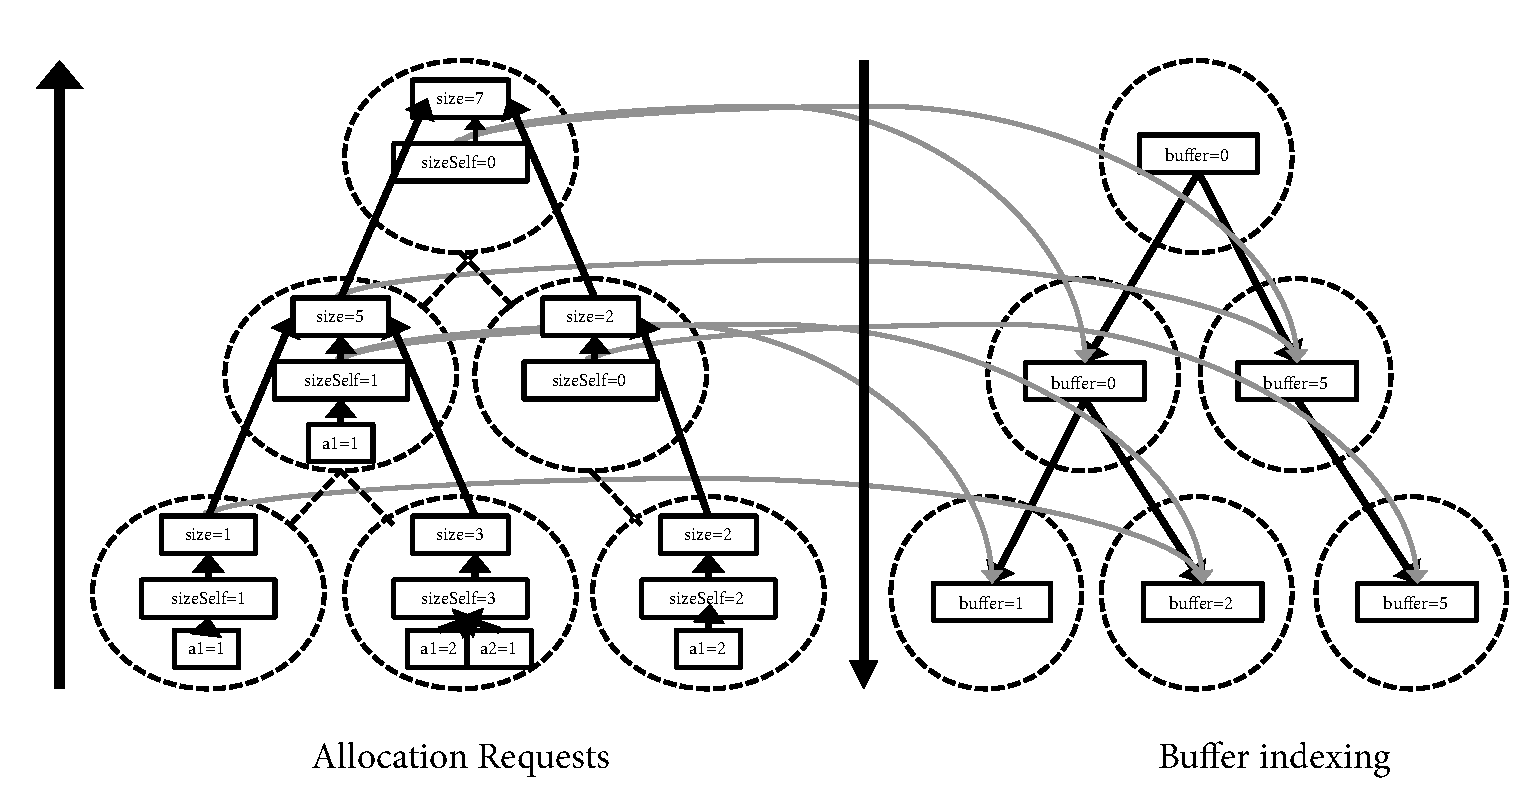
\includegraphics[trim=0 0 0 0,clip,width=1.0\columnwidth]{chapter6/macro}
\caption{\textbf{Staged parallel memory allocation as two tree traversals.} First pass is parallel bottom-up traversal computing the sum of allocation requests and the second pass is a parallel top-down traversal computing buffer indices. Lines with arrows indicate dynamic data dependencies.}
\label{fig:renderingtraversal}
\end{figure}


\subsection{Problem}
The static language of traversals is restricted, but we find that it can express important cases of typically more dynamic constructs. Prominent in our case studies, dynamic memory allocation provides significant flexibility for a language, but it is unclear how to perform it on a GPU without significant performance penalties. Our insight is that the memory allocation may be staged with parallel traversals by using a variant of prefix sum node labeling. One pass gathers  memory requests, a bulk allocation for the total amount is made, and then a scatter pass provides each node with a contiguous memory segment of it. We found manipulating memory addresses in this way to be error-prone, so we created two complementary automation techniques. First, we use our synthesizer to automatically schedule parallel memory allocation. Second, we syntactically hide the use of our optimization through a macro that automatically expands into staged dynamic memory allocation and consumption calls.

For example, we found parallel dynamic memory allocation to simplify the transition between layout and rendering. All nodes that render a circle will call some form of \code{drawCircle} in Figure~\ref{fig:stagedalloc:original}. Depending on the size of the circle, which is computed as part of the layout traversals, a different amount of memory will be allocated. Once the memory is allocated, vertices will be filled in with the correct position. The rendering engine will then connect the vertices with lines and paint them to the screen. The processing of converting the abstract shape into renderable vertices is known as tessellation. We want our system to tesselate the display objects for each node in parallel.




\subsection{Staged Parallel Memory Allocation}
We stage the use of dynamic memory into four logical phases: 
\begin{enumerate}
\item Parallel request (bottom-up tree traversal to gather )
\item Physical memory allocation
\item Parallel response (top-down tree traversal to scatter)
\item Computations that consume dynamic memory (normal parallel tree traversals)
\end{enumerate}
 The staging allows us to parallelize the request and response stages. We reuse the parallel tree traversals for them, as well as for the actual consumption. The actual allocation of physical memory in stage 2 is fast because it is a single call. Figure~\ref{fig:renderingtraversal} shows the dynamic data dependencies and two parallel tree traversals for an instance of staged parallel memory allocation.

Library functions that requires dynamic memory allocation are manually rewritten into allocation request  (Figure~\ref{fig:stagedalloc:alloc}) and memory consumption fragments (Figure~\ref{fig:stagedalloc:Render}). The transformation was not onerous to perform on our library primitives and, in the future, might be automated. 

Invocations of the original in the attribute grammar are rewritten to use the new primitives. For example, drawing two circles (Figure~\ref{fig:stagedallocClient:original}) is split into calls for allocation requests, buffer pointer manipulation, and buffer usage (Figure~\ref{fig:stagedallocClient:expanded}). The transformation increases memory consumption costs due to book keeping of allocation sizes. 

The result of our staging is three logical parallel passes, which, in practice, is merged into two parallel passes over the tree. The first pass is bottom up, similar to a prefix sum: each node computes its allocation requirements, adds that to the allocation requirements of its children,and then the process repeats for the next level of the tree. The \code{sizeSelf} and \emph{size} attributes are used for the first pass. Once the cumulative memory needs is computed, a bulk memory allocation occurs, and then a parallel top-down traversal assigns each node a memory span from \code{buffer} to \code{buffer + selfSize}. Finally, the memory can be used for actual computations through normal parallel passes. Memory use can occur immediately upon computation of the buffer index, so the last two logical stages are merged in implementation.

\subsection{Automation with Automatic Scheduling and Macros}
Manually manipulating the allocation requests and buffer pointers is error prone. We eliminated the problem through two automation techniques: automatic scheduling to enforce correct parallelization and macro expansion to encapsulate buffer manipulation.

To enforce proper parallelization, we relied upon our synthesizer to schedule the calls. If the synthesizer cannot schedule allocation calls and buffer propagation, it reports an error. Our insight is that, implicit to our staged representation, we could faithfully abstract the memory manipulations as foreign function calls. Our synthesizer simply performs its usual scheduling procedure.

To encapsulate buffer manipulation, we introduced the macro '@'.  Code that uses it is similar to code that assumes dynamic memory allocation primitives: the slight syntactic difference can be seen between Figure~\ref{fig:stagedallocClient:macro}  and Figure~\ref{fig:stagedallocClient:original}. Our macros (implemented in OMetaJS~[[CITE]]) automatically expand into the form seen in Figure~\ref{fig:stagedallocClient:expanded}. 

Our use case only required one allocation stage, but multiple may be needed.  For example, a final logging stage might be added that should run after all other computations, including rendering. However, the '@' calls described above expand to contribute to one attribute (\code{size}): no allocation is made until all of the sizes are known, which prevents making an allocation after using dynamic memory. To support multiple allocation stages, the '@' macro could be expanded to include logical group names: \code{@[render]Circle(...)} would contribute to \code{sizeRender}, \code{@[log]error(...)} to \code{sizeLog}, and \code{@[render,log]Strange(...)} to both \code{sizeRender} and \code{sizeLog}. Parallel traversals would be created for each logical name, and the synthesizer would be responsible for determining if the traversals can be merged in the final schedule and implementation.



\section{Scheduling Loops}


\section{Evaluation: Layout as Structured Parallel Visits}
\subsection{Box model}
\subsection{Nested text}
\subsection{Grids}


\subsection{SIMD Rendering through Staged Memory Allocation}
We evaluate three dimensions of our staged memory allocation approach: flexibility, productivity, and performance. First, it needs to be able to express the rendering tasks that we encounter in GPU data visualization. Second, it should some form of productivity benefit for these tasks. Finally, the performance on those tasks must be fast  enough to support real-time animations and interactions of big data sets.



\subsubsection{Productivity}
Productivity is difficult to measure. Before using the automation extensions for rendering, we repeatedly encountered bugs in manipulating the allocation calls and memory buffers. The bugs related both to incorrect scheduling and to incorrect pointer arithmetic. Our new design eliminates the possibility of both bugs.

One suggestive productivity measure is of how many lines of code the macro abstraction eliminates from our visualizations. We measured the impact on using it for 3 of our visualizations. The first visualization is our HBox language extended with rendering calls, while the other two are interactive reimplementations of popular visualizations: a treemap~[[CITE]] and multiple 3D line graphs~[[CITE]].


\begin{table}[ht]
\caption{Lines of Code Before/After Invoking the '@' Macro}
\centering
\begin{tabular}{c r r r}
\hline\hline
 \textbf{Visualization} & \textbf{Before (loc)} & \textbf{After (loc)} & \textbf{Decrease} \\ [0.5ex] \hline
  HBox & 97 & 54 & 44\% \\
  Treemap & 296 & 241 & 19\% \\
  GE & 337 & 269 & 20\% \\ [1ex] 
\hline
\end{tabular}
\label{table:macroreduction}
\end{table}
Table~\ref{table:macroreduction} compares the lines of code in visualizations before and after we added the macros. Using the macros eliminated 19--44\% of the code. Note that we are \emph{not} measuring the macro-expanded code, but code that a human wrote.



As shown in Figure~\ref{fig:stagedallocClient}, the eliminated code is code that was introduced by staging the library calls. Porting unstaged functional graphics calls to the library, is in practice, an alpha renaming of function names.  Using the '@' macro eliminates 19--44\% of the code that would have otherwise been introduced and completely eliminates two classes of bugs (scheduling and pointer arithmetic), so the productivity benefit is non-trivial. 

\subsubsection{Performance}


\section{Related Work}
Lang of schedules
\begin{itemize}
\item background
\item stencils and skeletons: wavefront, ...
\item polyhedra
\end{itemize}
Schedule verification
\begin{itemize}
\item compare to OAG etc., looser dataflow/functional langs
\end{itemize}